%Параметры страницы для большей схожести с веб-версией
\documentclass[12pt]{article}
\usepackage[total={170mm,230mm}]{geometry}

\usepackage{cmap}
%\usepackage{hyperref}
\usepackage[utf8]{inputenc}
\usepackage[T2A]{fontenc}
\usepackage[russian]{babel}


\usepackage{graphicx}
\usepackage{xcolor}
\usepackage{amssymb}
\usepackage{amsmath}
\usepackage{physics}
\usepackage{wrapfig}
\usepackage{pdfpages}

\usepackage{pgfplots}
\pgfplotsset{width=7cm,compat=newest}

\usepackage{amsmath}
\DeclareMathOperator\arctanh{arctanh}

\usepackage{amsmath}
\DeclareMathOperator\arccosh{arccosh}

\usepackage{amsmath}
\DeclareMathOperator\const{const}

\title{Введение в математический анализ}
\author{Алексей Савватеев \and Александр Тонис}

\begin{document}
\maketitle
\begin{abstract}
В данной лекции рассмотрены некоторые примеры или сюжеты, помогающие понять такие основы математического анализа, как предел последовательности, дифференцирование и приближенное вычисление выражений. Кроме того, приведено простое геометрическое доказательство теоремы Пифагора.
	\par
Конспектировал Александр Козлов. 
\end{abstract}	
\tableofcontents
\newpage
\section{Как далеко видно с горы}

\subsection{Формулировка задачи}
Рассмотрим следующую задачу. Как далеко может видеть наблюдатель, находящийся на вершине горы высоты $h$? Землю считать шарообразной, влиянием воздуха пренебречь. 

\subsection{Строгое решение задачи}
Во\--первых, ясно, что конечность дальности обзора связанна с кривизной поверхности Земли: если бы планета была плоской, то в отсутствии воздуха ничто бы не препятствовало наблюдению сколь угодно далеких мест на её поверхности. Если наблюдатель смотрит в данном направлении, то его взор охватывает лишь ту часть поверхности Земли, что расположена ниже касательной, проведенной из его глаз к поверхности Земли. Точка касания соответствует точке на горизонте. 

\par
Во\--вторых, так как в рамках рассматриваемой задачи форма Земли полагается шарообразной, то становится не важным направление, в котором смотрит наблюдатель. В какую бы сторону он не посмотрел~\----~вид будет тот же самый. Поэтому можно рассматривать лишь сечение системы ''наблюдатель\--Земля'' плоскостью, проходящей через центр Земли и через касательную, соединяющую глаза наблюдателя с точкой на горизонте. Получаем обычную школьную геометрическую задачу.
\begin{figure}[!ht]
 \centering
 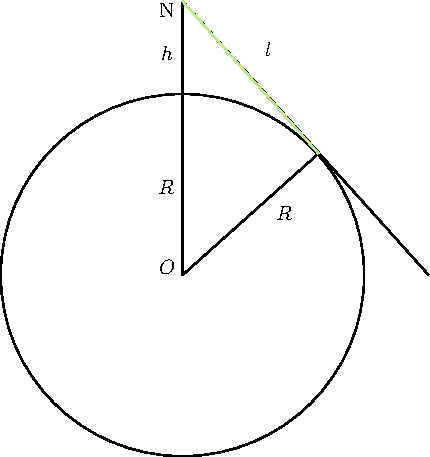
\includegraphics[width=0.5\textwidth]{first1.pdf}
 \caption{Чертёж к задаче о дальности обзора. Точка $N$ соответствует положению наблюдателя, точка $O$ отвечает центру Земли.}
 \label{fig:1}
\end{figure}
\par
Нужно найти расстояние $l$ (см. рис. \ref{fig:1}). Касательная, радиус Земли и отрезок, соединяющий наблюдателя с центром Земли, образуют прямоугольный треугольник, для сторон которого по теореме Пифагора справедливо:
\begin{equation}
 (R+h)^2 = R^2 + l^2.
\end{equation}
Из данного выражения нетрудно получить искомое расстояние:
\begin{equation}\label{eq:1}
 l = \sqrt{2Rh + h^2}.
\end{equation}

\subsection{Упрощение ответа}
Полученный результат может быть труден для запоминания. Зададимся вопросом о таком упрощении данной формулы, которое будет крайне слабо отражаться на ответе. То есть мы хотим упростить формулу (заменить её другой, более простой формулой) и не сильно при этом изменить ответ.

\par
Оценим входящие в формулу (\ref{eq:1}) величины. Радиус Земли $R$ равен примерно $6 370$ км, в то время как высота горы $h$ не может быть больше $9$ км (высота самой большой горы на Земле составляет 8 848 метров). Тогда выходит, что первое подкоренное слагаемое порядка десятков тысяч квадратных километров, а второе порядка десятков квадратных километров. Разумно пренебречь вторым слагаемым, ведь оно крайне слабо влияет на ответ. Оно даёт ошибку только в четвертом знаке, что зачастую не важно. Таким образом приходим к более простой формуле:
\begin{equation}
 l = \sqrt{2Rh}.
\end{equation}

Проиллюстрируем графиком (см. рис. \ref{fig:2}) тот факт, что используемое приближение и вправду не сильно меняет ответ. Видно, что точный и приближенный результаты почти не различимы. Если рассматривать зависимость от $h$, то видно, что она не линейная, а корневая, то есть если подняться в сто раз выше, то видно станет лишь в десять раз дальше.

\begin{figure}[htb]
 \centering
 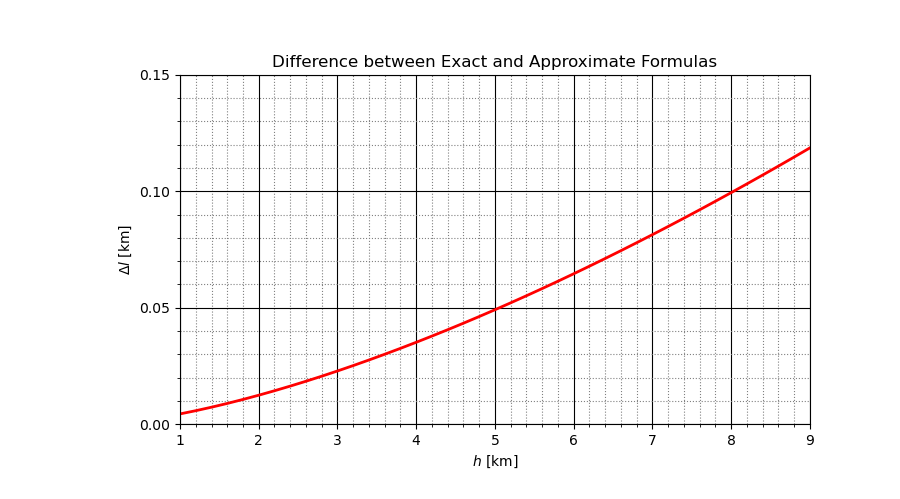
\includegraphics[width=\textwidth]{1.png}
 \caption{ Разница между точной и приближенной формулами расчета дальности обзора. Видно, что разница на интервале допустимых значений высот гор не больше 150 метров.}
 \label{fig:2}
\end{figure}

\par
Выходит, что мы упростили выражение, не потеряв его сути. Этим и занимается математический анализ~\----~разрабатывает методы упрощения выражений, исследует малые и большие величины, как с ними стоит обращаться.

\subsection{Геометрическое доказательство теоремы Пифагора}
Выше была использована теорема Пифагора, важно помнить её простое геометрическое доказательство. Пускай есть прямоугольный треугольник с катетами $a$ и $b$, а так же с гипотенузой $c$ (на чертежах ниже он выделен зеленым цветом). Рассмотрим квадрат со стороной $a+b$. Сперва разобьем его на два квадрата со стороной $a$ и со стороной $b$ и на 4 исходных треугольника таким образом, как показано на первом чертеже (см. рис. \ref{fig:31}). Получаем, что площадь большого квадрата есть сумма площадей квадратов поменьше ($a^2+b^2$) и четырех площадей исходного треугольника.
\begin{figure}[ht]
	\centering
	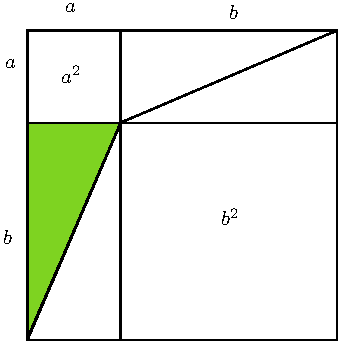
\includegraphics[width=0.5\textwidth]{first21.pdf}
	\caption{Чертёж к доказательству теоремы Пифагора. Первое разбиение квадрата. Зеленым выделен исходный прямоугольный треугольник.}
	\label{fig:31}
\end{figure}

\par
Теперь разобьем квадрат так, как показано на втором чертеже (см. рис. \ref{fig:32}). То есть сначала строим четыре прямоугольных треугольника, как показано на чертеже. Затем замечаем, что получившийся из их гипотенуз ромб на самом деле является квадратом, ведь, например, развернутый угол $\angle AQD$ состоит из углов $\angle AQP$ и $\angle MQD$, сумма которых равна девяноста градусам по свойству прямоугольного треугольника, а так же из угла $\angle PQM$, которому ничего не остается, кроме как быть прямым (аналогичные рассуждения справедливы для каждого из углов четырехугольника $QPLM$). То есть получилось, что площадь большого квадрата есть сумма площадей четырех прямоугольных треугольников и площади квадрата со стороной $c$. Ясно, что площадь большого квадрата в том и другом случаях остается неизменной; тогда
\begin{equation}
 a^2 + b^2 + 4S_\triangle=c^2+4S_\triangle.
\end{equation}
Если сократить площади треугольников, то получим соотношение, называемое теоремой Пифагора:
\begin{equation}
 a^2 + b^2 =c^2.
\end{equation}
На этом доказательство теоремы завершено.
\begin{figure}[ht]
	\centering
	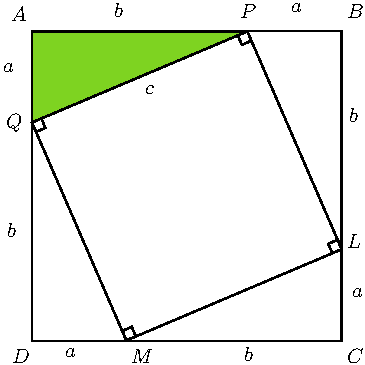
\includegraphics[width=0.5\textwidth]{first22.pdf}
	\caption{Чертёж к доказательству теоремы Пифагора. Второе разбиение квадрата. Зеленым выделен исходный прямоугольный треугольник.}
	\label{fig:32}
\end{figure}
\section{Вычисление массы Земли}
Рассмотрим несколько сюжетов, с помощью которых можно будет проиллюстрировать такое важное для математического анализа понятие, как дифференцирование. 

\par
Рассмотрим пример о приближенном вычислении массы Земли. Пускай по некоторым физическим величинам производятся расчеты, но данные физические величины были измерены с ошибкой. Как эта ошибка отразится на результате расчетов?

\subsection{Вычисление объема Земли}
Обозначим за $R$ \emph{измеренное значение радиуса Земли}. Из\--за наличия ошибки измерений можно утверждать, что \emph{фактический радиус Земли} есть $R+\Delta R$, где за $\Delta R$ обозначена \emph{ошибка измерений радиуса Земли}. Как же эта ошибка повлияет на вычисленный объем земного шара (Земля полагается шарообразной)? Из школьного курса стереометрии должна быть известна формула объема шара:
\begin{equation}\label{eq:6}
 V = \dfrac43 \pi R^3.
\end{equation}
Обозначим через $V$ измеренный объем земного шара (он вычисляется по измеренному радиусу). А фактический объем Земли обозначим через $V + \Delta V$, где  за $\Delta V$ обозначена \emph{ошибка вычислений объема Земли}. Тогда по той же формуле объема шара пишем:
\begin{equation}\label{eq:7}
 V + \Delta V = \dfrac43 \pi \qty(R + \Delta R)^3.
\end{equation}
Отсюда требуется найти $\Delta V$. Если вычесть из уравнения (\ref{eq:7}) уравнение (\ref{eq:6}), то получим:
\begin{equation}
\begin{split}
    \Delta V &= \dfrac43 \pi \qty(\qty(R + \Delta R)^3 - R^3)\\
    &=\dfrac43 \pi \qty(3R^2\Delta R + 3R \Delta R^2 + \Delta R^3)\\
    &= 4 \pi R^2\Delta R \qty( 1 + \dfrac{\Delta R}{R} +\dfrac{1}{3} \qty[\dfrac{\Delta  R}{R}]^2 ).
\end{split}
\label{eq:8}
\end{equation}
В итоговом виде равенства можно какими-то слагаемыми пренебречь. Например, измерили мы радиус Земли с точностью $1\%$, тогда в большой скобке выражения (\ref{eq:8}) стоит сумма трех величин:
\begin{equation}
 1 + \dfrac{1}{100} + \dfrac{1}{3}\dfrac{1}{10000}.
\end{equation}
Видно, что второе и третье слагаемые гораздо меньше первого, поэтому ими можно пренебречь. Тогда можно приближенно записать:
\begin{equation}\label{eq:10}
 \Delta V \approx 4 \pi R^2\Delta R.
\end{equation}
Эта формула имеет простой геометрический смысл (см. рис. \ref{fig:4}). Синим обозначен земной шар в представлении тех, кто измерял его радиус, желтой штриховкой обозначен тонкий шаровой слой~\----~отличие измеренного земного шара от фактического. Объем этого шарового слоя обозначается за $\Delta V$. Если ошибка измерений радиуса мала, то площадь одной из поверхностей шарового слоя приближенно можно вычислить как объем прямоугольного параллелепипеда с площадью основания, равной площади сферы $4 \pi R^2$, и высотой $\Delta R$. Тогда и получаем формулу (\ref{eq:10}).
\begin{figure}[!ht]
 \centering
 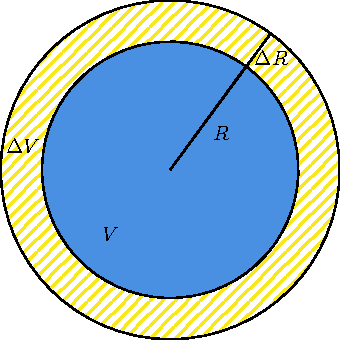
\includegraphics[width=0.5\textwidth]{first3.pdf}
 \caption{Геометрическая аналогия к задаче об объеме Земли.}
 \label{fig:4}
\end{figure}

\subsection{Завершение вычисления массы Земли}
Для того, чтобы определить массу планеты, нужно умножить среднюю плотность планеты на её объем. С последним мы уже разобрались. Средняя плотность Земли может быть измерена в ходе специальных экспериментов. Пускай через $\rho$ обозначено \emph{измеренное значение средней плотности Земли}, через $\rho + \Delta \rho$ обозначим \emph{фактическое значение средней плотности Земли}, где $\Delta \rho$~\----~\emph{ошибка измерения}. Тогда \emph{измеренная масса} $M$ будет равна
\begin{equation}
 M = \rho V.
\end{equation}
\emph{Фактическая масса} $M + \Delta M$ будет вычисляться по формуле
\begin{equation}
 M + \Delta M = \qty(\rho + \Delta \rho) \qty(V + \Delta V).
\end{equation}
Тогда ошибка вычисления массы Земли будет определяться выражением
\begin{equation}
 \Delta M = \Delta \rho \Delta V + \Delta \rho V + \rho \Delta V .
\end{equation}
Первое слагаемое является малым по сравнению с остальными, им можно пренебречь. Можно показать малость данного слагаемого геометрической аналогией (см. рис. \ref{fig:5}). Рассмотрим прямоугольник со сторонами $V$ и $\rho$. Его площадь будет равна измеренной массе Земли $M$. Тогда ошибки измерений можно представить как маленькие добавки к сторонам прямоугольника. Добавка к площади прямоугольника разбивается на три, площадь самого малого из добавочных прямоугольников соответствует слагаемому $\Delta \rho \Delta V$. Это показывает разумность пренебрежения им. Таким образом мы получаем:
\begin{equation}\label{eq:14}
 \Delta M \approx \Delta \rho V + \rho \Delta V.
\end{equation}
\begin{figure}[!ht]
 \centering
 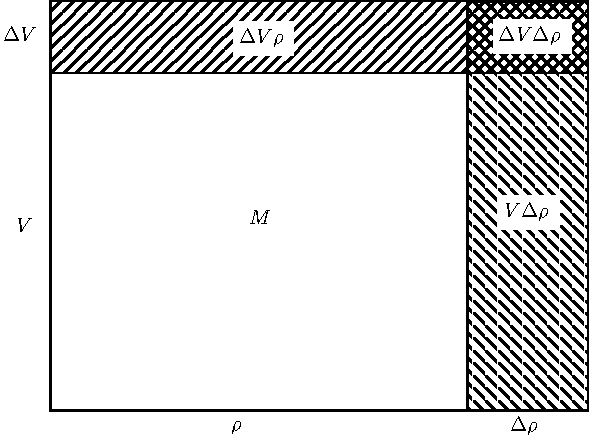
\includegraphics[width=0.8\textwidth]{first4.pdf}
 \caption{Геометрическая аналогия к задаче о массе Земли}
 \label{fig:5}
\end{figure}

\subsection{Комментарии о значении полученных результатов}
Теперь приведем несколько комментарием о значениях этих формул для понимания математического анализа. Первая приближенная формула (\ref{eq:10}) для ошибки вычисления объема земного шара представляет собой частный случай \emph{формулы производной от степенной функции}. Чтобы не давать строгих определений, запишем общую формулу в виде приближенного равенства:
\begin{equation}
 \Delta\qty(x^n) \approx n x^{n-1} \Delta x.
\end{equation}
Она читается: <<Приращение функции $x^n$ есть произведение $nx^{n-1}$ на приращение $x$>>. В нашем случае $n=3$ и добавлен несущественный множитель $4\pi$.
\par
Вторая приближенная формула (\ref{eq:14}) есть не что иное, как \emph{правило дифференцирования произведения}. То есть приращение произведения двух величин есть сумма двух слагаемых: произведения приращения первой величины на вторую и произведения приращения второй величины на первую.
\par
Попробуем то же самое записать в терминах относительной погрешности. Относительная погрешность есть отношение абсолютной погрешности к измеренной величине. Например, относительная погрешность измерения радиуса:
\begin{equation}
 \varepsilon_R = \dfrac{\Delta R}{R}.
\end{equation}
Для объёма получаем:
\begin{equation}
 \varepsilon_V = \dfrac{\Delta V}{V} = 3 \dfrac{\Delta R}{R} = 3 \varepsilon_R.
\end{equation}
Для массы относительная погрешность будет:
\begin{equation}
 \varepsilon_M = \dfrac{\Delta M}{M} = \dfrac{\Delta \rho}{\rho} + \dfrac{\Delta V}{V}.
\end{equation}
То есть относительная погрешность произведения двух величин равна сумме их относительных погрешностей.

\subsection{Немного цифр}
Рассмотрим численные значения физических величин, чтобы лучше понимать, о чём шла речь ранее. Радиус Земли можно оценить, как:
\begin{equation}
 R = 6.4 \vdot 10^6 \text{м} \pm 1\%.
\end{equation}
То есть относительная погрешность измерения радиуса Земли составляет $1\%$.
Для плотности Земли имеем:
\begin{equation}
 \rho = 5.5 \tfrac{\text{т}}{\text{м}^3} \pm 1\%.
\end{equation}
Тогда для объёма Земли получаем:
\begin{equation}
 V = 1.1\vdot10^{21}\text{м}^3 \pm 3\%.
\end{equation}
Для массы Земли справедлив следующий ответ:
\begin{equation}
 V = 6.05\vdot10^{21}\text{т} \pm 4\%.
\end{equation}

\section{Треугольники и окружности}
\subsection{Постановка задачи}
В данном сюжете мы затронем вопрос о пределе последовательности. Рассмотрим следующую задачу. Пускай задан любой треугольник с некоторыми углами $\alpha_0$, $\beta_0$ и $\gamma_0$ (см. рис. \ref{fig:6}). В него можно вписать единственным образом окружность. На точках касания вписанной окружности сторон треугольника строим следующий треугольник. Его углы обозначаем теми же буквами, что и противолежащие углы большего треугольника, но с индексами большими на единицу. Затем снова вписываем в данный треугольник с углами $\alpha_1$, $\beta_1$ и $\gamma_1$ окружность и по точкам касания вписанной окружности сторон треугольника строим следующий треугольник с углами $\alpha_2$, $\beta_2$ и $\gamma_2$ и так далее. Можно заметить, что треугольники становятся с каждым шагом более похожи на равносторонние. Покажем, что действительно имеет место подобное стремление.

\begin{figure}[!ht]
	\centering
	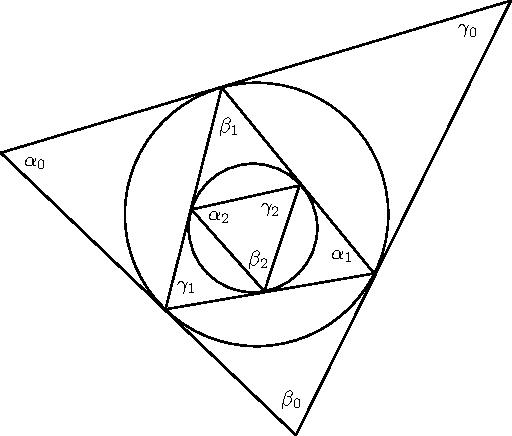
\includegraphics[width=0.8\textwidth]{first5.pdf}
	\caption{Чертёж к задаче о вписанных в треугольники окружностях}
	\label{fig:6}
\end{figure}

\subsection{Формальное геометрическое решение}
 Для этого рассмотрим любой треугольник $ABC$ с углами $\alpha_0$, $\beta_0$ и $\gamma_0$ (см. рис. \ref{fig:7}). Обозначения для точек касания приведены на чертеже. Из свойств касательных к окружности следует, что треугольники $AMK$ и $BNM$ являются равнобедренными. Из свойства равнобедренного треугольника получаем, что углы при основании равны
\begin{equation}
	\angle AMK = \angle MKA, \quad \angle BNM = \angle NMB.
\end{equation}
Так как сумма углов треугольника равна $180^{\circ}$, то отсюда можно найти углы при основании равнобедренных треугольников:
\begin{equation}
	\angle AMK = 90^{\circ} - \dfrac{\alpha_0}{2}, \quad \angle NMB = 90^{\circ} - \dfrac{\beta_0}{2}.
\end{equation}
Но угол $\angle AMB$ является развёрнутым, поэтому
\begin{equation}\label{eq:25}
	\gamma_1 = 180^{\circ} - \qty(90^{\circ} - \dfrac{\alpha_0}{2}) - \qty(90^{\circ} - \dfrac{\beta_0}{2}) = \dfrac{\alpha_0 + \beta_0}{2}.
\end{equation}
Ясно, что аналогичные соотношения справедливы и для других углов треугольника $MNK$:
\begin{equation}\label{eq:26}
	\alpha_1 = \dfrac{\gamma_0 + \beta_0}{2}, \quad \beta_1 = \dfrac{\gamma_0 + \alpha_0}{2}.
\end{equation}
Такую же связь можно получить для углов первого и второго треугольников, второго и третьего треугольников и так далее. Поэтому можно записать в общем виде:
\begin{equation}
	\quad \alpha_{n+1} = \dfrac{\gamma_n + \beta_n}{2}, \quad \beta_{n+1} = \dfrac{\gamma_n + \alpha_n}{2}, \quad \gamma_{n+1} = \dfrac{\alpha_n + \beta_n}{2}.
\end{equation}
\begin{figure}[!ht]
	\centering
	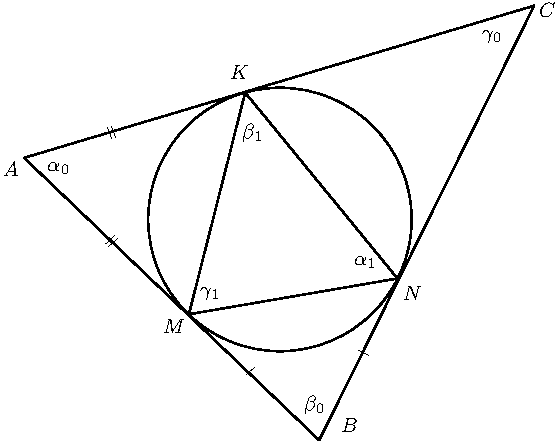
\includegraphics[width=0.8\textwidth]{first6.pdf}
	\caption{Чертёж к нахождению связи между углами нулевого и первого шага}
	\label{fig:7}
\end{figure}
\subsection{Завершение доказательства}
Отложим углы на числовой прямой. Без ограничения общности будем полагать
\begin{equation}
	\alpha_0 < \beta_0 < \gamma_0.
\end{equation}
Прежде всего отложим углы $\alpha_0$, $\beta_0$ и $\gamma_0$ (см. рис. \ref{fig:8}). Затем по полученным формулам (\ref{eq:25}) и (\ref{eq:26}) определяем положение следующего набора углов. $\alpha_1$ будет лежать посередине между $\beta_0$ и $\gamma_0$, $\gamma_1$ будет лежать посередине между $\alpha_0$ и $\beta_0$, $\beta_1$ будет лежать посередине между $\alpha_0$ и $\gamma_0$.
\par
Тут можно заметить, что расстояние между углами $\alpha_1$ и $\gamma_1$ уменьшилось в два раза по сравнению с расстоянием между углами $\alpha_0$ и $\gamma_0$. Действительно:
\begin{equation}
	\gamma_1 - \alpha_1 = \dfrac{\alpha_0 + \beta_0}{2} - \dfrac{\beta_0 + \gamma_0}{2} = \dfrac{\alpha_1- \gamma_1 }{2}.
\end{equation}
Таким образом, разница между самым большим и самым маленьким углом новой последовательности в два раза меньше разницы между самым большим и самым маленьким углом предыдущей последовательности.
\begin{figure}[!ht]
	\centering
	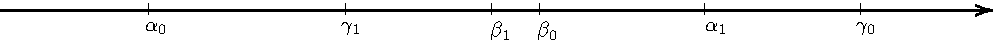
\includegraphics[width=\textwidth]{first7.pdf}
	\caption{Числовая прямая с углами}
	\label{fig:8}
\end{figure}
\par
Данный результат можно обобщить следующим образом:
\begin{equation}\label{eq:30}
	\abs{\alpha_{n+1} - \gamma_{n+1}} = \dfrac{\abs{\alpha_{n} - \gamma_{n}}}{2}.
\end{equation}
Если начать с углов $\alpha_0$, $\beta_0$ и $\gamma_0$, последовательно применяя формулу (\ref{eq:30}) $n$ раз, то получится связь
\begin{equation}
	\abs{\alpha_{n+1} - \gamma_{n+1}} = \dfrac{\abs{\alpha_{0} - \gamma_{0}}}{2^n}.
\end{equation}
Отсюда видно, что если применять формулу очень много раз, то интервал возможных значений углов будет сужаться около $60^{\circ}$ (потому что интервал возможных значений $\alpha$, $\beta$ и $\gamma$ сжимается в точку в то время, как их сумма должна оставаться равной $180^{\circ}$).
\subsection{Пример}
Продемонстрируем данный вывод на примере треугольника с сильно разными углами:
\begin{equation}
	\alpha_{0} = 16^{\circ},\quad \beta_0 = 20^{\circ}, \quad \gamma_0 = 144^{\circ}.
\end{equation}
Тогда уже на седьмом шаге получим, что разброс значений, которые могут принимать углы $\alpha_7$, $\beta_7$ и $\gamma_7$, составляет всего лишь $1^{\circ}$:
\begin{equation}
	\abs{\alpha_{7} - \gamma_{7}} = \dfrac{16^{\circ} - 144^{\circ}}{2^7} = 1^{\circ}.
\end{equation}
То есть на седьмом шаге получается треугольник сильно похожий на равносторонний.
\end{document}
